% Title: gl2ps_renderer figure
% Creator: GL2PS 1.4.2, (C) 1999-2020 C. Geuzaine
% For: Octave
% CreationDate: Fri Sep 10 20:09:21 2021
\setlength{\unitlength}{1pt}
\begin{picture}(0,0)
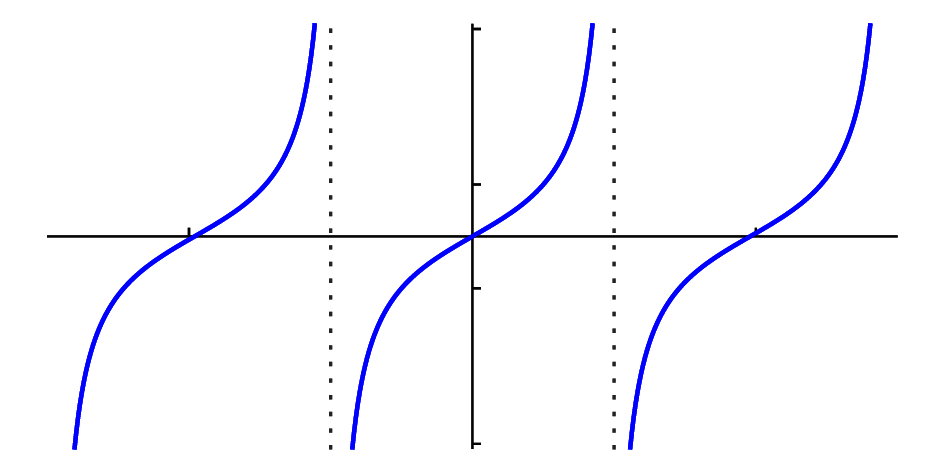
\includegraphics[width=8cm,height=4cm]{fig_functions_tan}
\end{picture}%
\begin{picture}(226,113)(0,0)
\fontsize{10}{0}\selectfont\put(45.3543,48.8036){\makebox(0,0)[t]{\textcolor[rgb]{0.15,0.15,0.15}{{$-\pi$}}}}
\fontsize{10}{0}\selectfont\put(181.417,48.8036){\makebox(0,0)[t]{\textcolor[rgb]{0.15,0.15,0.15}{{$\pi$}}}}
\fontsize{10}{0}\selectfont\put(108.384,6.52794){\makebox(0,0)[r]{\textcolor[rgb]{0.15,0.15,0.15}{{-4}}}}
\fontsize{10}{0}\selectfont\put(108.384,43.8623){\makebox(0,0)[r]{\textcolor[rgb]{0.15,0.15,0.15}{{-1}}}}
\fontsize{10}{0}\selectfont\put(108.384,68.7519){\makebox(0,0)[r]{\textcolor[rgb]{0.15,0.15,0.15}{{1}}}}
\fontsize{10}{0}\selectfont\put(108.384,106.086){\makebox(0,0)[r]{\textcolor[rgb]{0.15,0.15,0.15}{{4}}}}
\fontsize{10}{0}\selectfont\put(161.027,106.086){\makebox(0,0)[l]{\textcolor[rgb]{0,0,0}{{$\tan(x)$}}}}
\fontsize{10}{0}\selectfont\put(212.031,50.0847){\makebox(0,0)[l]{\textcolor[rgb]{0,0,0}{{$x$}}}}
\end{picture}
